\chapter{Technologie}

Tato kapitola představuje důležité technologie a přístupy použité v rámci této práce.

\section{Solid.js}

Solid.js\footnote{\url{https://solidjs.com}} je JavaScriptová knihovna pro tvorbu uživatelských rozhraní obdobně jako React, Vue, nebo Svelte.


\subsection{Rozdíly}

Rozdíl mezi Solid.js a ostatními knihovnami spočívá v technologii synchronizování změn v \gls{dom}.

Populární knihovny jako React, nebo Vue používají tzv. \gls{vdom}, což je virtuální reprezentace \gls{dom} stromu v paměti, která se porovnává s reálným \gls{dom} stromem a rozdíly mezi nimi se aplikují pomocí diffing algoritmu.

Solid.js a nově i Svelte používají granulární, reaktivní modely pro sledování změn v \gls{dom}.
Prakticky Solid.js využívá principu “dependency tracking”, kde přístupy k reaktivním proměnným jsou sledovány tzv. “subscribers”, kteří jsou upozornění na případné změny respektive zápisy do těchto proměnných~\cite{solid-reactivity}.
Tento princip připomíná designový vzor “Observer”.

\subsection{Rychlost}

Tabulka~\ref{tab:technology1} porovnává Solid.js s vybranými frameworky.
Všechny metriky jsou vypočítané na příkladové aplikaci \gls{todomvc}\footnote{\url{https://todomvc.com}} implementované v daném frameworku, aby test byl spravedlivý.
Každé skóre je číslo normalizované do intervalu <1, $\infty$), které nám říká velikost zhoršení oproti nejlepší implementaci~\cite{krausest120,krausest122}.

První metrika ``Operations'' je vážený geometrický průměr skóre všech operací nad příkladovou aplikací (např. vytvoření řádku, smazání řádku, vybraní řádku a další\dots).

Druhá metrika ``Transferred size'' je vážený geometrický průměr skóre přenesených dat po síti při použití daného frameworku.

Poslední metrika ``Memory allocation'' je vážený geometrický průměr skóre využití paměti.

% % TODO: Different background color for table

\begin{table}[ht]
      \begin{ctucolortab}
            \begin{tabular}{c c c c c}
                  \bfseries Metrika & \bfseries{Solid 1.8.0} & \bfseries{Svelte 5} & \bfseries{Vue 3.3.6} & \bfseries{React 18.2.0} \\\Midrule{}
                  Operations        & \textbf{1.08}          & 1.08                & 1.24                 & 1.53                    \\
                  Transferred size  & \textbf{2.29}          & 3.04                & 7.16                 & 15.32                   \\
                  Memory allocation & \textbf{1.45}          & 1.52                & 2.13                 & 2.81
            \end{tabular}
      \end{ctucolortab}
      \caption{Porovnání rychlosti Solid.js s populárními frameworky}
      \label{tab:technology1}
\end{table}

Z výsledku benchmarku můžeme vidět, že Solid.js obdobně jako Svelte je velice blízko 1, tedy je jenom o 8\% pomalejší než nejrychlejší implementace.
Svelte od verze 5 má obdobný styl reaktivivního modelu jako Solid.js, což vysvětluje podobné výsledky~\cite{svelte-reactivity}.

% \section{Svelte}\label{sec:Svelte}

% Svelte je kompilátor pro tvorbu uživatelských rozhraní obdobně jako populární alternativy React, nebo Vue.
% Každá komponenta se nachází v souboru s příponou ``.svelte'' a podobně jako Vue obsahuje tři části:

% \begin{itemize}
%     \item \textbf{Script tag} --- obsahuje logiku komponenty v JavaScriptu.
%     \item \textbf{Style tag} --- obsahuje styly komponenty.
%     \item \textbf{Template} --- obsahuje html kód komponenty.
% \end{itemize}

% \subsection{Rozdíly}

% Mezi hlavní rozdíly Svelte oproti jiným frameworkům patří:

% \begin{itemize}
%     \item \textbf{Kompilátor} --- Největší rozdíl oproti zmíněným frameworkům se vyskytuje v tom, že Svelte není runtime, který se posíla na klienta společně se zdrojovým kódem komponent.
%           Svelte je kompilátor souborů s příponou ``.svelte'', který převede komponenty na optimalizovaný imperativní kód v JavaScriptu.
%     \item \textbf{Reaktivita} --- Svelte používá reaktivní model pro změny v \gls{dom} namísto \gls{vdom}.
%     \item \textbf{Podpora komunity} --- Svelte není produktem velkých společností jako je React od Meta Platforms, nebo Angular od Google.
%           Zároveň už to není čistě produkt autora Riche Harrise a komunity, ale od roku 2021 je vývoj plně sponzorován platformou Vercel.
%     \item \textbf{Vývojářská přívetivost (DX)} --- Svelte je v praxi jednodušší na používání a intuitivní i pro nové vývojáře.
% \end{itemize}

% Kompilátor s sebou nese jednu nevýhodu a to je velikost výsledného kódu po kompilaci.
% Prázdný projekt ve Svelte má minimální velikost, protože zde není potřeba téměř žádného imperativního kódu pro zaručení reaktivity.
% To vede k tomu, že každá nová komponenta přidává unikátní kus kódu a zvyšuje tak velikost dat, které se posílají přes internet na klienta.
% Existuje tak inflexní bod, kdy velikost aplikace bude vyšší než aplikace napsané v Reactu.
% V praxi se však ukazuje, že toto může být potenciálně problémové pouze u velkých aplikací s velkým počtem komponent~\cite{svelte-scaling}.
% \subsection{VDOM vs Reaktivita}

% Důležitý rozdíl mezi Svelte a podobnými frameworky je ten, že neobsahuje \gls{dom} diffing algoritmus jako to je u Reactu.
% Veškeré změny v \gls{dom} jsou ve Svelte řešené pomocí reaktivních proměnných, které automaticky při své změně vyvolají změnu i ve zmíněném \gls{dom}.
% Sledování změn je zaručeno na základě vytvořeného imperativního kódu při kompilaci (viz. sekce~\ref{sec:Svelte} a ukázky kódu~\ref{svelte-counter} a~\ref{svelte-counter-compiled}).

% \begin{lstlisting}[caption={Počítadlo ve Svelte 4}, label={svelte-counter}, language=html]
% <script>
% 	let count = 0(*@\label{svelte-counter-2}@*)

% 	function add() {
% 		count++
% 	}
% </script>

% <button on:click={add}>+1</button>(*@\label{svelte-counter-9}@*)
% <p>Current count: {count}</p>(*@\label{svelte-counter-10}@*)
% \end{lstlisting}

% V ukázce kódu~\ref{svelte-counter} je důležitá deklarace proměnné \texttt{count} na řádku~\ref{svelte-counter-2}.
% Veškeré změny této proměnné jsou sledovány (viz. ukázka kódu~\ref{svelte-counter-compiled}).
% Na řádku~\ref{svelte-counter-9} je vidět přiřazený callback \texttt{add} na událost click.
% Následně můžeme vidět použití proměnné \texttt{count} na řádku~\ref{svelte-counter-10} v rámci textového uzlu elementu.

% \clearpage

% \begin{lstlisting}[caption={Počítadlo po kompilaci}, label={svelte-counter-compiled}, language=JavaScript]
% function instance($$self, $$props, $$invalidate) {
%     let count = 0;

%     function add() {
%         $$invalidate(0, count++, count);(*@\label{svelte-counter-compiled-5}@*)
%     }

%     return [count, add];
% }

% class App extends SvelteComponent {
%     constructor(options) {
%         super();
%         init(this, options, instance, create_fragment, safe_not_equal, {});
%     }
% }
% \end{lstlisting}

% V zjednodušené ukázce kódu~\ref{svelte-counter-compiled} je na řádku~\ref{svelte-counter-compiled-5} podstatné volání funkce \texttt{\$\$invalidate}, která zaručuje reaktivitu proměnné \texttt{count}.
% Každé přiřazení hodnoty je kompilátorem převedeno na volání funkce \texttt{\$\$invalidate}, které označí danou proměnnou jako změněnou a následně naplánuje její změnu včetně aktualizace elementů, kde se používá.

% \subsection{Rychlost}

% Tabulka~\ref{tab:technology1} ukazuje porovnání Svelte s vybranými frameworky.
% Všechny metriky jsou vypočítané na příkladové aplikaci \gls{todomvc} implementované v daném frameworku, aby test byl spravedlivý.
% Každé skóre je číslo normalizované do intervalu <1, $\infty$), které nám říká velikost zhoršení oproti nejrychlejší implementaci~\cite{krausest119,krausest120}.

% První metrika ``Operations'' je celkový vážený geometrický průměr skóre všech operací nad příkladovou aplikací (např. vytvoření řádku, smazání řádku, vybraní řádku a další\dots).

% Druhá metrika ``Startup metrics'' je vážený geometrický průměr skóre výsledků z \gls{lighthouse} testování.

% Poslední metrika ``Memory allocation'' je vážený geometrický průměr skóre využití paměti.

% % TODO: Different background color for table

% \begin{table}[ht]
%     \begin{ctucolortab}
%         \begin{tabular}{c c c c c}
%             \bfseries Metrika & \bfseries{Svelte 5} & \bfseries{Svelte 4} & \bfseries{Vue 3.3.6} & \bfseries{React 18.2.0} \\\Midrule{}
%             Operations        & 1.06                & \textbf{1.26}       & 1.22                 & 1.43                    \\
%             Startup metrics   & 1.06                & \textbf{1.02}       & 1.27                 & 1.67                    \\
%             Memory allocation & 1.48                & \textbf{1.36}       & 1.86                 & 2.45
%         \end{tabular}
%     \end{ctucolortab}
%     \caption{Porovnání rychlosti Svelte s populárními frameworky}
%     \label{tab:technology1}
% \end{table}

% Z výsledků můžeme vidět, že Svelte 4 je optimalizované velikostně pro start aplikace a využití paměti, což vychází z principu kompilátoru.
% V další kapitole se podívám na to, jak se mění princip Svelte v nové verzi 5, která přináší velké změny v architektuře Svelte.

\section{TypeScript}

JavaScript je dynamicky typovaný jazyk, což se v praxi ukázalo jako těžkopádné při škálování velkých projektů.
Postupem času existovaly různé nástroje a nadstavby nad samotným jazykem, které mu přidávali statické typování.
Nástroje jako TypeScript\footnote{\url{https://typescriptlang.org}}, Flow\footnote{\url{https://flow.org}}, nebo ReasonML\footnote{\url{https://reasonml.github.io}} se ukázaly jako vhodným řešením pro škálovatelnost, znovupoužitelnost a přehlednost kódu.
Pomyslným vítězem se v posledních letech ukázal TypeScript, který má vysokou popularitu i podporu v rámci ekosystému, proto není náhodou, že ho ve své práci plně používám.
TypeScript dodává znovupoužitelným komponentám větší přehlednost při zpětném čtení kódu, ale i konzumenti komponent mají k dispozici robustní typovou kontrolu včetně fungujícího automatického doplňování kódu.

\section{Distribuce komponent}

\begin{itemize}
      \item \textbf{Knihovna komponent} je taková knihovna komponent, která už má předepsané styly. Většinou je možnost přepsat většinu stylů pomocí ``themes'', ale HTML kód komponent je téměř vždy neměnitelný.
            Hodně se stává, že vývojáři potřebují odlišnou HTML strukturu než je dána.
            Častým případem je právě řešení přístupnosti, kdy je potřeba přidat elementy navíc do komponenty pro např. správné fungování čteček obrazovky.
            \begin{lstlisting}[caption={Ukázka použití komponentové knihovny}, label={component-distribution}, language=html]
import { Button } from "component-library"

export const Dashboard = () => {
      return (
            <div>
                  <Button>Open file</Button>
            </div>
      )
}
\end{lstlisting}
      \item \textbf{Knihovna headless komponent} se liší od klasické knihovny komponent tím, že neobsahuje předepsané styly.
            Zde můžeme rozlišit dvě různé úrovně headless komponent.
            \begin{itemize}
                  \item Exportující jednotlivé prvky komponenty, konzument tak má větší kontrolu nad výsledným kódem komponenty.
                        Ovšem HTML struktura v jednotlivých prvcích komponent není stále plně flexibilní.
                  \item Exportující pouze logiku v podobě ``primitiv''. V Reactu se jedná o ``custom hooks'', ve Vue ``composition utilities'', ve Svelte to jsou prosté funkce, které pracují s reaktivními proměnnými a obdobně i ve Solid.js.
            \end{itemize}
      \item \textbf{Copy and paste} není klasická knihovna.
            Tato varianta vznikla jako reakce na headless komponenty a primitiva.
            Jedná se o způsob distribuce komponent, kde konzumenti si zkopírují předpis komponenty.
            Využívá tak existujících headless komponent, nebo UI primitiv.
            Tato varianta je velmi flexibilní, protože umožňuje distributorům přidávat vzorové styly, které konzument může smazat, nebo vyměnit za vlastní řešení.
            Zároveň má konzument plnou kontrolu nad kódem komponenty.
            Nevýhodou je horší znovupoužitelnost a zároveň nutnost manuální aktualizace komponenty pokud se změní její logika.
            Distribuce takových komponent je většinou v podobě \gls{cli}, nebo zkopírováním z dokumentace.
\end{itemize}

\begin{lstlisting}[caption={Ukázka použití headless knihovny}, label={component-distribution-2}, language=html]
import { Tab } from "headless-component-library"

export const Toolbar = () => {
  return (
    <Tab.Group>
      <Tab.List className="flex flex-col gap-4">
        <Tab>
          {({ selected }) => (
            <button
              className={
                selected ? 'bg-blue-500' : 'bg-white'
              }
            >
              Tab 1
            </button>
          )}
        </Tab>
      </Tab.List>
      <Tab.Panels>
        <Tab.Panel>Content 1</Tab.Panel>
      </Tab.Panels>
    </Tab.Group>
  )
}
\end{lstlisting}

\clearpage

V porovnání všech tří přístupů na obrázku~\ref{component-lib-distribution-comparison} můžeme vidět, že vyšší flexibilita přináší i vyšší úroveň abstrakce.
To znamená, že čím flexibilnější je API komponenty, tím více času je potřeba pro pochopení, použití a údržbu komponent.

Knihovny komponent jsou nejvýhodnější, pokud není potřeba vlastního brand designu a zároveň jsme spokojení s úrovní přístupnosti, kterou nám komponenta dodává.

Headless komponenty jsou lepší v situacích, kde potřebujeme zasáhnout významně do designu (kaskádových stylů) komponenty pro vlastní potřeby.
Nicméně se tím navyšuje i čas strávený na vývoji.

UI primitiva jsou nejvýhodnější při budování vlastního designového systému, kde potřebujeme plnou kontrolu nad kódem komponenty.

Copy and paste přístup je nejvýhodnější, pokud chceme to nejlepší ze všech přístupů.
Flexibilitu headless komponent případně UI primitiv a zároveň rychlost vývoji jako při použití knihovny komponent.

\begin{figure}[h]
      \centering
      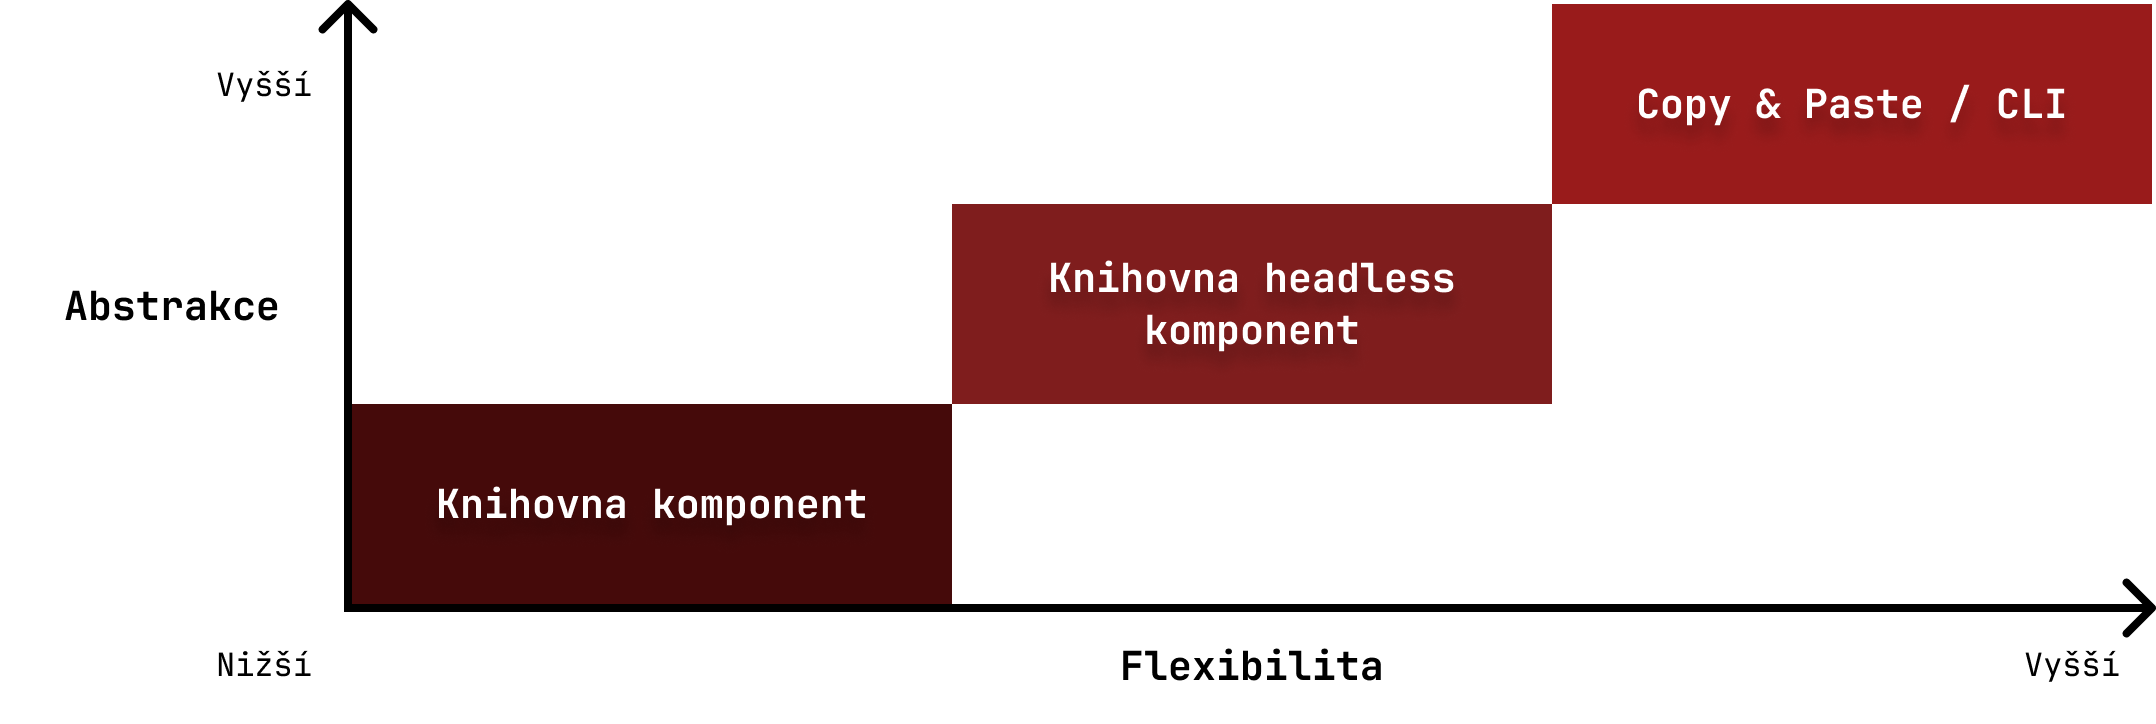
\includegraphics[width=\textwidth]{./assets/figures/component-lib-distribution-comparison.png}
      \captionsetup{justification=centering}
      \caption{Diagram abstrakce a flexibility různých přístupu k distribuci komponent}
      \label{component-lib-distribution-comparison}
\end{figure}

\clearpage

\section{Závěr technologií}

Tato kapitola popsala nejdůležitější technologie a přístupy, které jsou využity v rámci této práce.
Plná funkčnost celého projektu je závislá na dalších důležitých technologiích, které zde nejsou popsány neboť nejsou přímo relevantní k problematice tvorby znovupoužitelných komponent.

Samotná knihovna bude psána stylem UI primitiv, tedy funkcí v Solid.js, které vrací \gls{apg} logiku jako props a reference.
Taková knihovna může poté sloužit jako základ pro tvorbu designových systémů a knihoven (headless) komponent.

Solid.js knihovnu jsem zvolil ze dvou důvodů:

\begin{enumerate}
      \item Její ekosystém knihoven je stále v raních fázích a podobná knihovna respektive její části zde chybí.
      \item Solid.js má unikátní vlastnosti, které ho odlišují od ostatních knihoven.
            Hlavně co se týče performance a reaktivity.
            Tato knihovna má potenciál zlepšit a optimalizovat uživatelská rozhraní.
\end{enumerate}

TypeScript je velice důležitý pro nové knihovny, neboť usnadňuje budoucí údržbu kódu a vývojářskou přívětivost.
Ve světě webového vývoje je TypeScript dnes už téměř standardem a jeho nepoužití by vedlo k výrazně snížené adopci knihovny komunitou vývojářů~\cite{stateofjs-2022}.

% Sebek review:
% TODO: Zaver dane kapitoly (proc to Svelte atp.)
% TODO: Diagramy
% TODO: Porovnat se starym zpusobem komponent (v cem je to flexibilnejsi, modifikovatelnejsi?)
% TODO: Jakým způsobem to hodlám řešit
% Je to složitější na přečtení a zorientování (ten můj text), tak to zjednodušit, zpřehlednit.
